\section{Background and Context}

\subsection{First Principles Analysis of Energy Loss in an average car}
The force acting longitudinally on a vehicle can be modeled by the following : 

[TODO : figure with axis and gravity]
[]
\[
m\cdot a = F_{\text{motor}} - F_{\text{drag}} - F_{\text{roll}} + F_{\text{gravity}}
\]
where:
\begin{itemize}
    \item \textbf{Aerodynamic Drag:} 
    \[
    F_{\text{drag}} = \frac{1}{2} \rho\, C_d\, A\, v^2,
    \]
    with \(\rho\) being the air density, \(C_d\) the drag coefficient, \(A\) the frontal area, and \(v\) the vehicle speed.
    \item \textbf{Rolling Resistance:} 
    \[
    F_{\text{roll}} = C_{rr}\, m\, g,
    \]
    where \(C_{rr}\) is the rolling resistance coefficient, \(m\) the vehicle mass, and \(g\) the gravitational acceleration.
    \item \textbf{Gravitational Component:} 
    \[
    F_{\text{gravity}} = m\, g\, \sin\theta,
    \]
    representing the component of gravity along the road when the vehicle is on an slope with angle \(\theta\). this term become positive when we go downhill, the slope's angle $\theta$ is defined as negative downhill and positive uphill.
    \item \textbf{Force from motor Acceleration/Braking} 
    \[
    F_{\text{motor}}
    \]
    this term model the force by the motor/brake
\end{itemize}

Energy can be defined as a force endured over a distance. Similarly, power can be defined as a force endured at a given speed. Energy efficiency in this context can be defined by the amount of energy required to move by a given distance. Funny enough, this can also be brought back to a force. We will not address "the what" being moved for now, even tho it usually makes sense to also take into account "the what" in the form of cargo/ passenger in the efficiency to compare fairly a train and a car.

Vehicle Energy efficiency, measured as energy [kilo Watt Hour] per 100 [kilometer] as a function of speed (the others parameters usually remain nearly constant while travelling)

\begin{equation}
\eta(v) = \frac{1}{36}\cdot\left( \frac{1}{2}\,\rho\,C_d\,A\,v^2 + C_{rr}\,m\,g + m\,g\,\sin\theta \right) \quad \text{[kWh/100km]}.
\label{eq:energy_consumption}
\end{equation}


This gives an idea of what we can tune to minimize the amount of energy per unit of distance. Naturally, this model simplifies the reality by ignoring the energy wasted due to the acceleration/braking/idling cycle due to, e.g., a red light or the increased drag from wind. It also ignores the embodied energy in the vehicle.

\subsection{acceleration braking regime (city) and cruise regime losses}

To model more accurately the efficiency of a vehicle, we must factor the different driving condition and their relative weight over an average trip. A vehicle can be modelled with four distinct driving mode : Cruising, accelerating, braking and idling. There is fair amount of research studying theses driving modes and their relative proportion [TODO ADD citation china study, ]. It's hard to obtain a definite number for the proportion of each driving cycle as they depend on many parameters like the 

\begin{figure}[h]
    \centering
    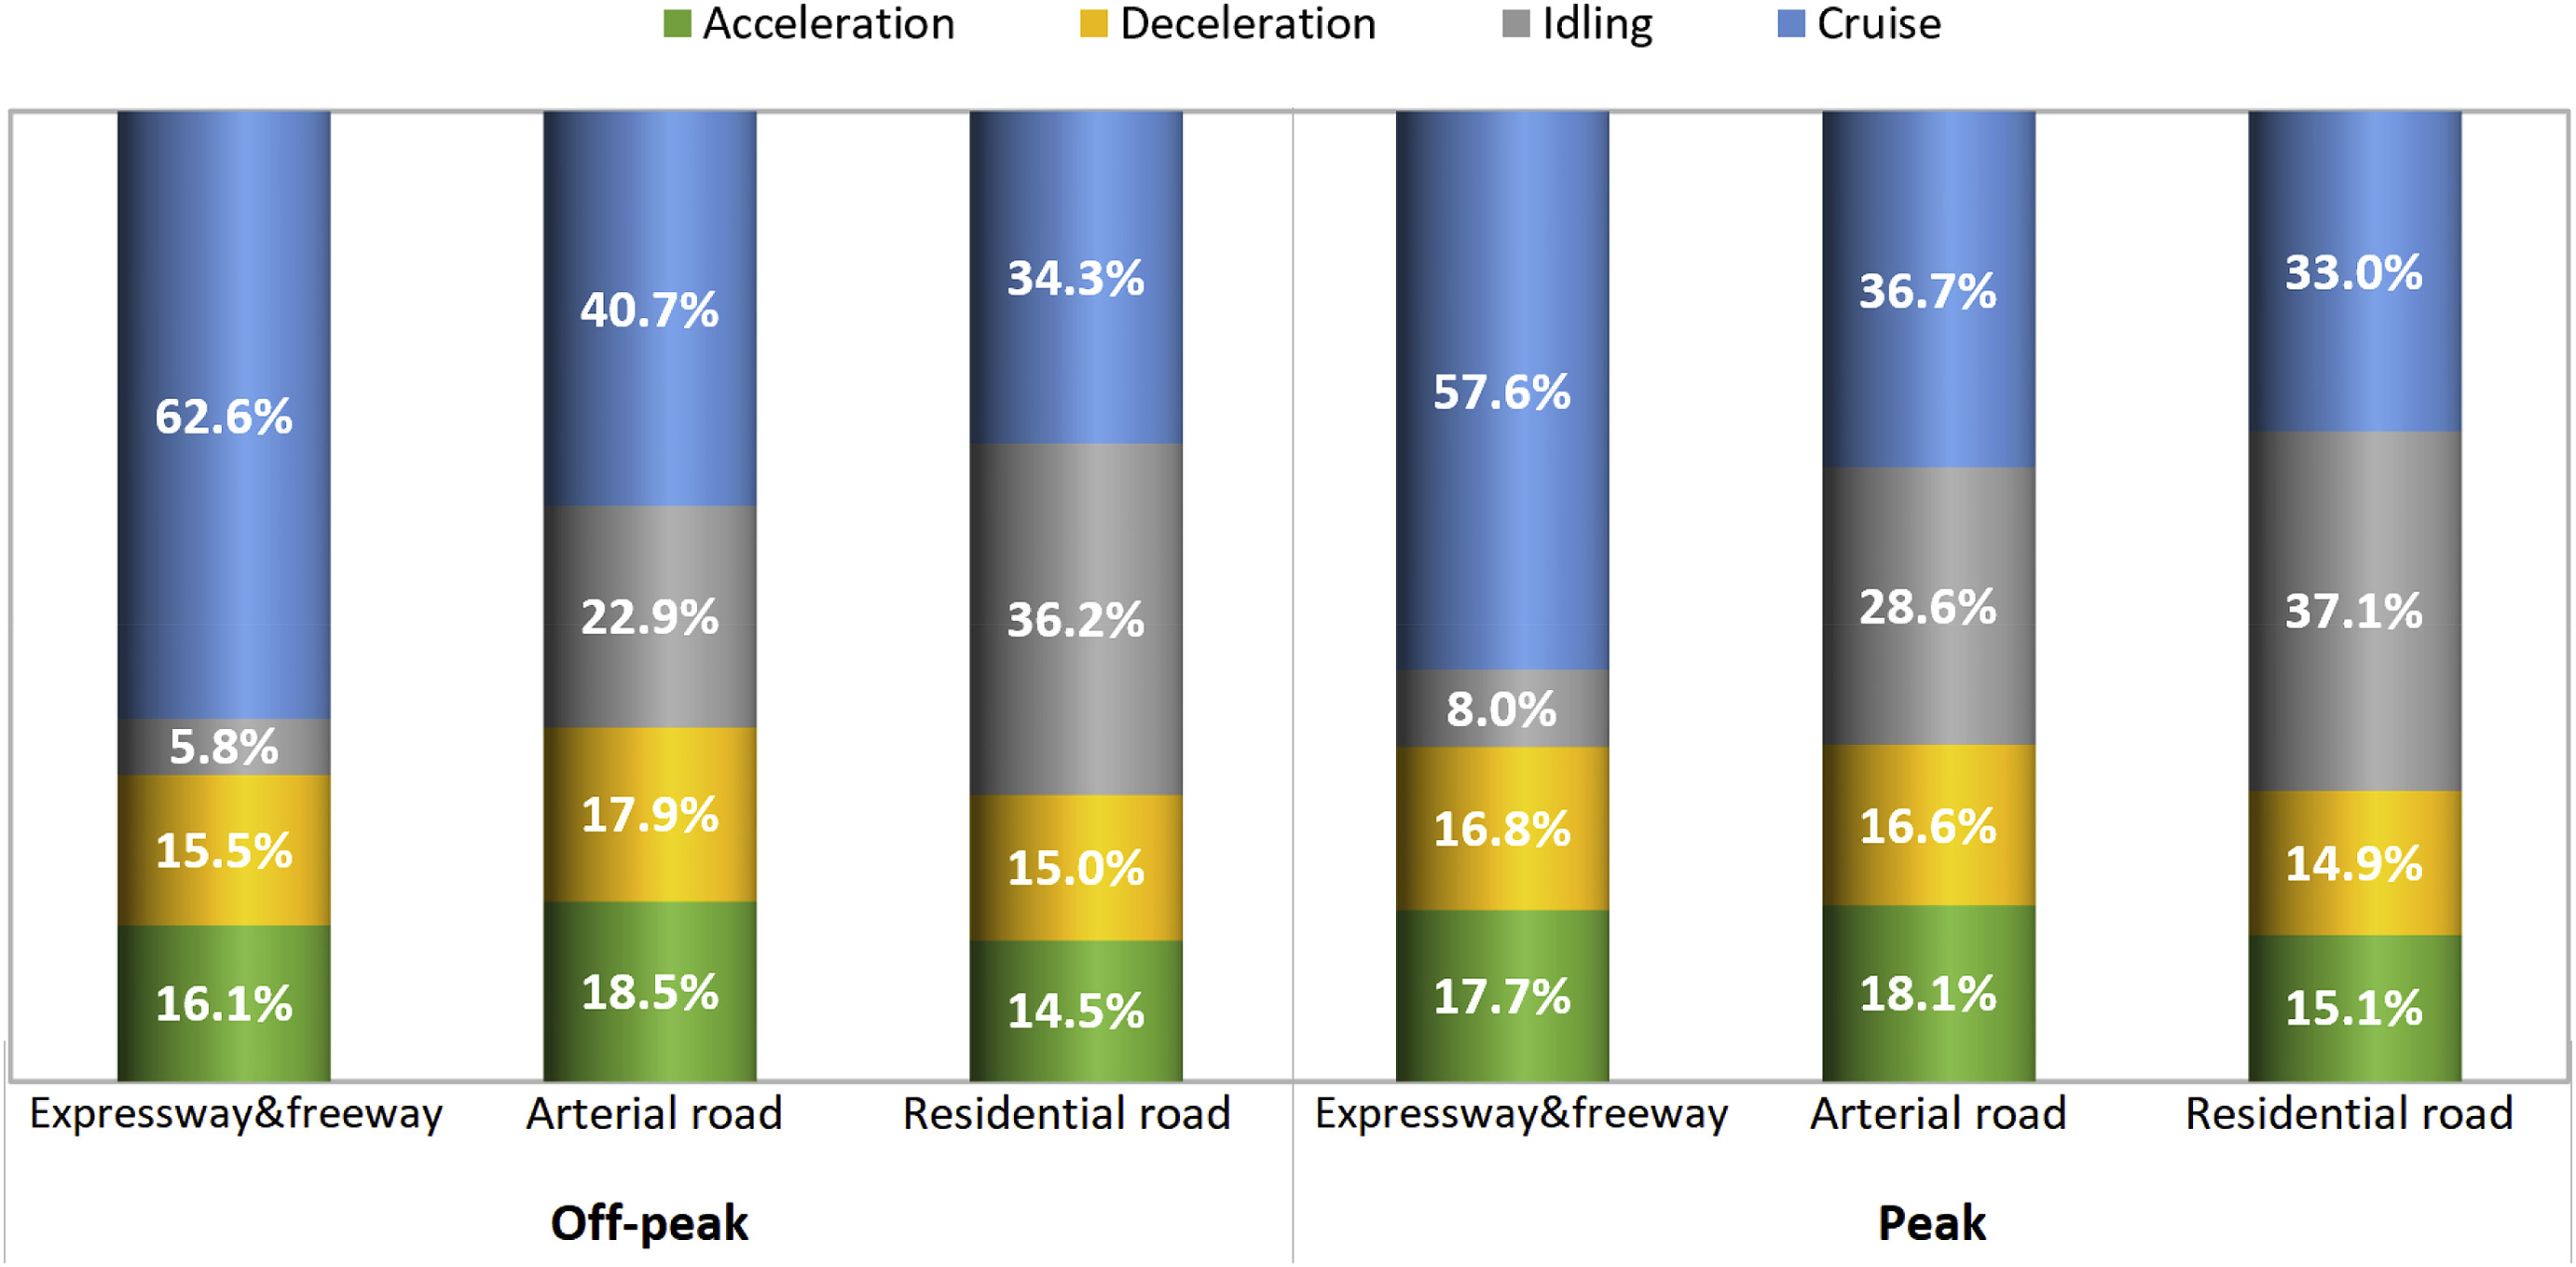
\includegraphics[width=0.8\linewidth]{Figures/ch2_shareOfDrivingModeChina.jpg}
    \caption{Figure from [CITE china study here] showing the relative proportion of driving mode}
    \label{fig:ch2proportiondrivingmode}
\end{figure}

also get some number on the acceleration braking amount and quantity (how much and how many)

we can conclude by noting that no driving mode is negligible in proportion.

we can define an idling efficiency (even tho the vehicle is not moving and thus only wasting energy, some will waste more energy per unit of time than others)

we can define a deceleration efficiency, measuring how much energy we can recover while braking (0\% for a typical ICE vehicle up to XX\% for an electric vehicle with regenerative braking) 

we can define an acceleration efficiency by looking at how much energy is wasted from the tank/battery to the wheel/kinetic energy.

It's also interesting to look at the speed profile on road to define how fast a car need to go and the tradeoff between trip time and speed.


\subsection{Importance of Mass and Aerodynamics in Energy Efficiency}

From the previous equations \eqref{eq:energy_consumption}, we see that to improve the efficiency we must minimize the mass and frontal area of the vehicle followed by a reduction of $C_d$ and $C_{rr}$.

\subsection{Importance of embodied Energy and material impact}
how much energy to build the vehicle, how much ressources

\subsection{Comparison with existing vehicle}

look at velomobile, twizi, smart, tesla, suv, small car, bike
get number on kwh/100km, embodied energy, typical speed, mass, frontal area, Cd, C_rr

